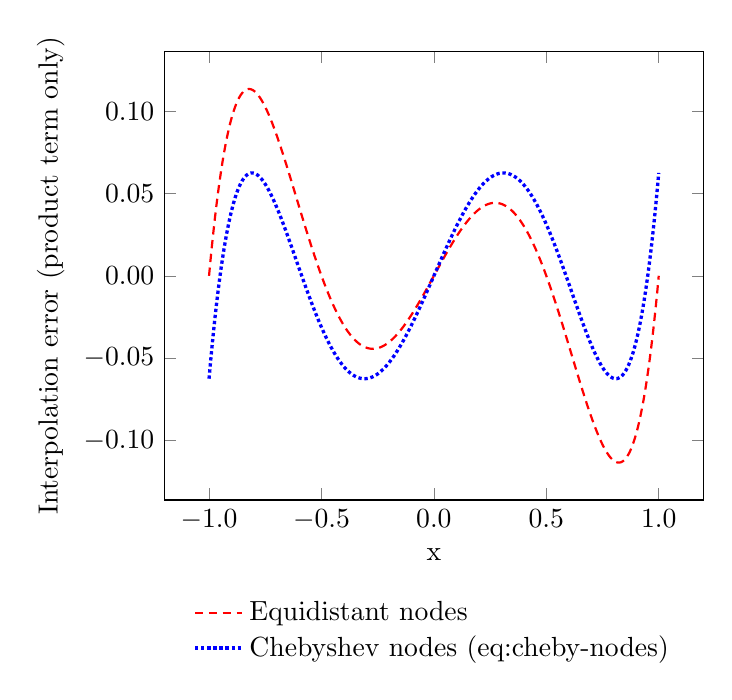
\begin{tikzpicture}

    \begin{axis}[
       scaled ticks=false,
       xlabel = x,
       ylabel = {Interpolation error (product term only)},
       ylabel near ticks,
       yticklabel style={/pgf/number format/.cd,fixed,precision=2, fixed zerofill},
       xticklabel style={/pgf/number format/.cd,fixed,precision=1, fixed zerofill},
       legend entries={Equidistant nodes, Chebyshev nodes (\eq{eq:cheby-nodes})},
       legend style={at={(0.5,-0.2)}, anchor=north, draw=none},
       legend cell align = left
    ]
    
      \addplot[red, densely dashed, thick, domain = -1:1, samples = 300] {(x+1)*(x+0.5)*x*(x-0.5)*(x-1.0)};
      \addplot[blue, densely dotted, very thick, domain = -1:1, samples = 300] {(x+0.95106)*(x+0.58779)*x*(x-0.58779)*(x-0.95106)};
  
    \end{axis}
\end{tikzpicture}